\documentclass[10pt]{beamer}

\usetheme{Madrid}
\usecolortheme{default}
\setbeamertemplate{navigation symbols}{}
\setbeamersize{text margin left=0.6cm,text margin right=0.6cm}

\usepackage{tikz}
\usetikzlibrary{automata, positioning, arrows.meta, shapes.geometric, shapes.arrows, fit, calc, matrix}
\usepackage{amsmath, amssymb}
\usepackage{booktabs}
\usepackage{array}

\newcolumntype{L}[1]{>{\raggedright\arraybackslash}p{#1}}
\pdfstringdefDisableCommands{\def\translate#1{#1}}

\newcommand{\ATM}{A_{\mathrm{TM}}}
\newcommand{\HALTTM}{\mathrm{HALT}_{\mathrm{TM}}}
\newcommand{\ETM}{E_{\mathrm{TM}}}
\newcommand{\RE}{\mathrm{RE}}
\newcommand{\coRE}{\mathrm{coRE}}

\title{Turing Machines, Undecidability, and Complexity}
\subtitle{Foundations of Computability and Intractability}
\author{Computer Science Theory}
\date{Slide Set 7}

\begin{document}

\begin{frame}
  \titlepage
\end{frame}

\begin{frame}{Learning Objectives}
  \small
  By the end of this slide set, you should be able to:
  \begin{itemize}
    \item connect CFGs/PDAs to context-sensitive grammars and bounded-tape machines;
    \item define a Turing machine (TM), configuration, recognizer, and decider;
    \item design a TM using implementation-level and high-level descriptions;
    \item explain why common TM variants have the same computational power;
    \item distinguish decidable, recognizable, and unrecognizable languages;
    \item prove undecidability using diagonalization and mapping reductions;
    \item apply Rice's theorem correctly; and
    \item distinguish computability from complexity, especially $P$, $NP$, and NP-completeness.
  \end{itemize}
\end{frame}

\begin{frame}{Road Map}
  \tableofcontents
\end{frame}

% ==========================================
% Part 1: The Standard Turing Machine
% ==========================================
\section{From CFGs and PDAs to CSGs and LBAs}

\begin{frame}{Why Go Beyond Pushdown Automata?}
  \small
  A PDA has unbounded memory, but it can access that memory only in LIFO order.
  This restriction prevents a PDA from recognizing some simple-looking languages, such as
  \[
    \{a^n b^n c^n \mid n\ge 0\}
    \qquad\text{and}\qquad
    \{ww \mid w\in\{0,1\}^*\}.
  \]
  \begin{block}{An intermediate step: change access before removing the bound}
    Replace the stack by a read--write tape whose usable length is bounded
    by the input length. A linear bounded automaton (LBA) can revisit and
    mark input cells, while still using only linearly bounded workspace.
  \end{block}
  \begin{alertblock}{Important distinction}
    The issue is not simply ``three blocks'' or ``a stack matches only two
    things.'' A stack can check arbitrarily many \emph{nested} obligations.
    The arrangement of dependencies, not just their number, matters.
  \end{alertblock}
\end{frame}

\begin{frame}{Context-Sensitive Grammars: Rewriting in Context}
  \small
  Use $G=(V,T,S,P)$, with finite disjoint variable and terminal sets.
  A context-sensitive production has the form
  \[
    \alpha A\beta\to\alpha\gamma\beta,
    \qquad A\in V,\quad \gamma\in(V\cup T)^+,
    \quad \alpha,\beta\in(V\cup T)^*.
  \]
  It replaces $A$ only in the specified surrounding context, which remains
  unchanged. For example, $aB\to abB$ applies to a $B$ preceded by $a$.
  \begin{block}{Equivalent language-level definition}
    \textbf{Noncontracting grammars} use rules $u\to v$ where $u$ contains
    a variable and $|u|\le|v|$. They generate exactly the same language
    family as context-sensitive grammars, though individual rule forms differ.
    The length-preserving rule $CB\to BC$ illustrates the distinction.
  \end{block}
  We allow $S\to\varepsilon$ only when $S$ never occurs on a right-hand
  side. A \textbf{CSL} is a language generated by such a grammar.
  The equivalence and this empty-word convention are discussed in~\cite{gallier-csg}.
\end{frame}

\begin{frame}{Linear Bounded Automata: A Precise Convention}
  \small
  An LBA is a tape machine confined between two protected endmarkers:
  \[
    B=(Q,\Sigma,\Gamma,\delta,q_0,\vdash,\dashv,F),\qquad
    \delta:(Q\setminus F)\times\Gamma
       \to\mathcal P(Q\times\Gamma\times\{L,R\}).
  \]
  Here $Q,\Sigma,\Gamma$ are finite, $q_0\in Q$, $F\subseteq Q$, and
  $\Sigma\subseteq\Gamma$. The distinct markers lie in $\Gamma\setminus\Sigma$.
  The initial tape is $\vdash w\dashv$, with the head at the left marker.
  \begin{itemize}
    \item The $|w|$ interior cells may be overwritten, but the head never
      moves outside the marked interval.
    \item Markers may neither be overwritten nor written into interior cells;
      at $\vdash$ only a right move is allowed, at $\dashv$ only a left move.
    \item Reaching $F$ halts and accepts; a nonfinal configuration with no
      move halts and rejects. A branch may also run forever.
  \end{itemize}
  Acceptance is existential over branches. A \emph{deterministic} LBA has
  at most one successor per state/symbol pair. Set-valued $\delta$ is
  essential for the general CSL correspondence.
\end{frame}

\begin{frame}{Worked LBA: Three Equal Blocks}
  \small
  \textbf{Goal:} recognize $L=\{a^n b^n c^n:n\ge1\}$ using only input cells.
  \begin{enumerate}
    \item Check $w\in a^+b^+c^+$; reject otherwise, including $\varepsilon$.
    \item From the left, mark the first unmarked $a$ as $X$.
    \item Continue right to the first unmarked $b$ and mark it $Y$;
      then find and mark the first unmarked $c$ as $Z$.
      Reject if a required match is missing.
    \item Return to $\vdash$ and repeat. When no $a$ remains, accept
      exactly when no unmarked $b$ or $c$ remains.
  \end{enumerate}
  \begin{block}{Snapshots after complete rounds, not individual transitions}
    \[
      \vdash aabbcc\dashv
      \ \Longrightarrow\ \vdash XaYbZc\dashv
      \ \Longrightarrow\ \vdash XXYYZZ\dashv.
    \]
    After $r$ successful rounds on $a^ib^jc^k$, the interior is
    $X^ra^{i-r}Y^rb^{j-r}Z^rc^{k-r}$. Thus acceptance forces $i=j=k$.
  \end{block}
  Every round marks three new cells; each sweep is bounded. This particular
  LBA is deterministic and halts on every input.
\end{frame}


\begin{frame}{The Bridge Theorem and the Next Step}
  \small
  \begin{block}{CSG--LBA correspondence \cite{gallier-csg}}
    A language is context-sensitive iff some \emph{nondeterministic} LBA
    accepts it, with the stated empty-word convention.
  \end{block}
  Allowing $c|w|$ work cells for a fixed constant $c$ is equivalent to the
  input-cell convention: encode a fixed number of tracks in each tape cell
  using a larger finite tape alphabet. Handle the empty input separately.
  \begin{itemize}
    \item Unlike the PDA, the LBA can revisit and rewrite all its usable cells.
    \item Unlike a general TM, it cannot use arbitrarily many fresh cells
      on one fixed input.
    \item A fixed input gives finitely many configurations, so searching
      their graph decides LBA acceptance. The appendix makes this precise.
  \end{itemize}
  Do not infer that deterministic and nondeterministic LBAs are equivalent:
  that remains an open problem~\cite{lba-notes}.
  \par\smallskip
  \textbf{Next:} remove the linear space restriction. A Turing machine may
  use any finite amount of tape during a finite computation---but even this
  model cannot decide every language.
\end{frame}

\section{The Standard Turing Machine}

\begin{frame}{A Standard Single-Tape Turing Machine}
  \begin{center}
  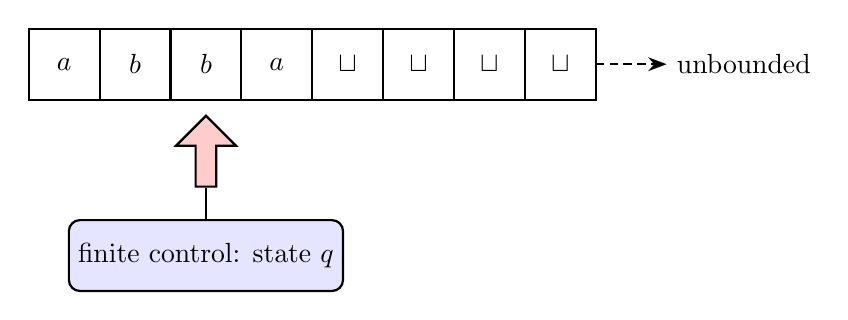
\begin{tikzpicture}[>=Stealth, thick, scale=0.9]
    \foreach \x in {0,...,7}{\draw (\x,0) rectangle +(1,1);}
    \node at (0.5,0.5) {$a$};
    \node at (1.5,0.5) {$b$};
    \node at (2.5,0.5) {$b$};
    \node at (3.5,0.5) {$a$};
    \node at (4.5,0.5) {$\sqcup$};
    \node at (5.5,0.5) {$\sqcup$};
    \node at (6.5,0.5) {$\sqcup$};
    \node at (7.5,0.5) {$\sqcup$};
    \draw[densely dashed,->] (8,0.5)--(9,0.5) node[right]{unbounded};

    \node[draw, fill=red!20, shape=single arrow, shape border rotate=90,
          minimum height=0.9cm] (head) at (2.5,-0.8) {};
    \node[draw, rounded corners, fill=blue!10, minimum width=3.2cm,
          minimum height=0.9cm] (control) at (2.5,-2.2) {finite control: state $q$};
    \draw (head.south)--(control.north);
  \end{tikzpicture}
  \end{center}
  \begin{itemize}
    \item The input occupies the leftmost cells; all remaining cells contain the blank $\sqcup$.
    \item In one step the machine reads, changes state, writes, and moves one cell left or right.
    \item We use the common one-way-infinite tape convention. Two-way-infinite tapes are equivalent.
    \item A left move at the leftmost cell leaves the head there.
  \end{itemize}
\end{frame}

\begin{frame}{Formal Definition: Convention Used Here}
  \small
  We use the Sipser-style halting-state convention throughout:
  \[
    M=(Q,\Sigma,\Gamma,\delta,q_0,q_{\mathrm{accept}},q_{\mathrm{reject}}),
  \]
  where
  \begin{itemize}
    \item $Q$ is a finite state set, containing distinct halting states
      $q_{\mathrm{accept}}$ and $q_{\mathrm{reject}}$;
    \item $\Sigma$ is a finite input alphabet and $\sqcup\notin\Sigma$;
    \item $\Gamma$ is a finite tape alphabet, with $\Sigma\subseteq\Gamma$ and $\sqcup\in\Gamma$;
    \item $q_0\in Q$ is the start state; and
    \item
      $\delta:(Q\setminus\{q_{\mathrm{accept}},q_{\mathrm{reject}}\})\times\Gamma
      \to Q\times\Gamma\times\{L,R\}$.
  \end{itemize}
  \begin{block}{Meaning of a transition}
    $\delta(q,a)=(p,b,R)$ means: in state $q$ scanning $a$, enter $p$, write $b$,
    and move one cell right.
  \end{block}
  The transition function is total on nonhalting states; entering either
  halting state ends the computation immediately.
  \footnotesize Linz often presents an equivalent final-state/partial-transition convention.
  The convention may change how halting is written, but not which languages can be recognized.
\end{frame}

\begin{frame}{Configurations (Instantaneous Descriptions)}
  \small
  A configuration records the current state, tape contents, and head position. We write
  \[
    uqv,
  \]
  where the head scans the first symbol of $v$, $u$ lies to its left, and $q$ is the current state.
  Trailing blanks are normally suppressed. If $v=\varepsilon$, the head
  scans the first implicit blank; $q_0\varepsilon$ starts on a blank cell.

  \begin{center}
  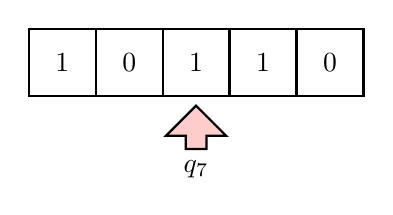
\begin{tikzpicture}[>=Stealth, thick, scale=0.85]
    \foreach \x in {0,...,4}{\draw (\x,0) rectangle +(1,1);}
    \node at (0.5,0.5) {1}; \node at (1.5,0.5) {0};
    \node at (2.5,0.5) {1}; \node at (3.5,0.5) {1}; \node at (4.5,0.5) {0};
    \node[draw,fill=red!20,shape=single arrow,shape border rotate=90,
          minimum height=0.55cm] at (2.5,-0.55) {};
    \node at (2.5,-1.1) {$q_7$};
  \end{tikzpicture}
  \end{center}
  The picture represents $10q_7110$. If $\delta(q_7,1)=(q_5,0,R)$, then
  \[
    10q_7110\ \vdash\ 100q_510.
  \]
  The initial configuration on $w$ is $q_0w$. A configuration containing
  $q_{\mathrm{accept}}$ or $q_{\mathrm{reject}}$ is halting.
\end{frame}


\begin{frame}{How to Describe a TM Without Drowning in Transitions}
  Following the standard textbook hierarchy, use the right level of detail:
  \begin{enumerate}
    \item \textbf{Formal description:} give all states and transitions. Best for small machines.
    \item \textbf{Implementation description:} describe head motions and tape operations in prose.
    \item \textbf{High-level description:} describe algorithmic stages, treating the tape as structured storage.
  \end{enumerate}
  \begin{block}{Design pattern: crossing off symbols}
    Repeatedly mark one symbol in each block, sweep back to the left, and verify that all blocks
    finish together. New tape symbols such as $X,Y,Z$ act as bookkeeping marks.
    A decorated first-cell symbol lets later sweeps locate the left end;
    returning there is a tape operation, not a free reset of the head.
  \end{block}
  \begin{alertblock}{A complete description must say}
    what happens on malformed input, when the machine accepts, and when it rejects.
    A decider must halt on every input.
  \end{alertblock}
\end{frame}

\begin{frame}{Worked Example: Deciding $\{0^n1^n\mid n\ge 0\}$}
  \small
  On input $w$:
  \begin{enumerate}
    \item First verify that $w\in 0^*1^*$; reject otherwise.
    \item Sweep from the left to find the first unmarked $0$; change it to
      $X$. If none remains, go to step 5.
    \item Sweep right to find the first unmarked $1$; change it to $Y$. If none exists, reject.
    \item Return to the left end and repeat.
    \item When no unmarked $0$ remains, accept iff no unmarked $1$ remains.
  \end{enumerate}
  \begin{block}{Tape snapshots on input $0011$}
    \[
      0011\ \Longrightarrow\ X0Y1\ \Longrightarrow\ XXYY\ \Longrightarrow\ \text{accept}.
    \]
  \end{block}
  On $0^i1^j$, after $r$ successful rounds the tape is
  $X^r0^{i-r}Y^r1^{j-r}$. Acceptance therefore forces $i=j$;
  conversely, equal counts complete every round. Every bounded sweep
  terminates, and each round marks new symbols. The empty word accepts.
\end{frame}

% The three-block marking example appears in the introductory LBA bridge.

% ==========================================
% Part 2: TM Variants and Robustness
% ==========================================
\section{TM Variants and Robustness}

\begin{frame}{Robustness of the TM Model}
  Many changes make programs easier to describe without changing which languages are recognizable.
  \small
  \begin{center}
  \begin{tabular}{L{2.2cm}L{3.2cm}L{3.4cm}}
    \toprule
    Variant & Computational power & Possible efficiency effect \\
    \midrule
    stay-put move $S$ & unchanged & constant-factor overhead \\
    two-way-infinite tape & unchanged & small simulation overhead \\
    multiple tapes/heads & unchanged & may be much faster \\
    nondeterminism & unchanged for computability & central to complexity \\
    enumerator & characterizes recognizable languages & different interface \\
    \bottomrule
  \end{tabular}
  \end{center}
  \begin{block}{Simulation principle}
    Show effective simulations in both directions. For recognizers,
    preserve the accepted language; for deciders, also ensure halting on
    every input. Enumerators require a separate interface-equivalence theorem.
  \end{block}
\end{frame}


\begin{frame}{Nondeterministic Turing Machines}
  \small
  An NTM may have several legal moves:
  \[
    \delta:(Q\setminus\{q_{\mathrm{accept}},q_{\mathrm{reject}}\})\times\Gamma
      \to \mathcal{P}(Q\times\Gamma\times\{L,R\}).
  \]
  It \textbf{accepts} an input if at least one computation branch accepts. It rejects only if all
  branches halt and reject; a blocked nonaccepting branch counts as rejection.
  A nondeterministic decider has no infinite branch.
  \begin{block}{Theorem}
    Every NTM has an equivalent deterministic TM.
  \end{block}
  \textbf{Proof sketch.}
  A DTM explores the NTM's computation tree breadth-first. Breadth-first search eventually reaches
  any accepting node; depth-first search may become trapped on one infinite branch.
  For an NTM decider, the search also terminates if no branch accepts.
  The finite-branching argument justifying this is in the appendix.
  \begin{alertblock}{Takeaway}
    Nondeterminism does not enlarge the class of computable languages, but it may change the
    resources needed. This distinction motivates $P$ versus $NP$.
  \end{alertblock}
\end{frame}

\begin{frame}{Universal Machines and Enumerators}
  \small
  \begin{block}{Universal Turing machine}
    A universal TM $U$ receives $\langle M,w\rangle$ and simulates machine $M$ on input $w$.
    Both programs and data are encoded as strings---the conceptual basis of stored-program computing.
  \end{block}
  \begin{block}{Enumerator}
    An enumerator is a TM with a printer. Starting from a blank tape, it prints strings over time;
    repetition and arbitrary order are allowed.
  \end{block}
  \begin{block}{Enumeration theorem}
    A language is Turing-recognizable iff some enumerator enumerates it.
  \end{block}
  \textbf{Proof idea.} A recognizer can be dovetailed over all inputs to produce an enumerator;
  conversely, compare the enumerator's outputs with the requested input.
\end{frame}

\begin{frame}{Encodings and Effective Simulation}
  \small
  Fix a finite alphabet, say binary, and a computable, unambiguous format
  for descriptions of machines, strings, and pairs. Write $\langle M,w\rangle$
  for the resulting encoded pair, not for a new input symbol.
  \begin{itemize}
    \item The simulator can decode a finite transition table and execute
      one simulated step effectively.
    \item A machine description can itself be input data. Thus
      $\langle M,\langle M\rangle\rangle$ is a legitimate encoded instance.
    \item Malformed descriptions are rejected by the standard machine
      acceptance/halting languages in this set. Their complements therefore
      include those malformed strings.
  \end{itemize}
  \begin{block}{Computing a string versus deciding a language}
    A TM with a designated output convention may compute a partial function
    $f:\Sigma^*\rightharpoonup\Sigma^*$. A decider instead computes a total
    yes/no membership function. Encoding a problem makes it precise;
    it does not guarantee that a TM can solve it.
  \end{block}
\end{frame}

% ==========================================
% Part 3: The Church--Turing Thesis
% ==========================================
\section{Decidability and the Church--Turing Thesis}

\begin{frame}{The Church--Turing Thesis}
  Church's $\lambda$-calculus and Turing's machines gave equivalent formal accounts of effective
  computation. Many other reasonable models were later shown equivalent as well.
  \begin{block}{Church--Turing thesis}
    Every function that is effectively calculable by an algorithm is Turing-computable.
  \end{block}
  It is a \emph{thesis}, not a mathematical theorem, because ``effective procedure'' is an informal
  notion rather than a previously defined mathematical object.
  \begin{alertblock}{Do not overstate it}
    The thesis identifies algorithmic computability with TM computability. Claims about what every
    physically possible device can compute are stronger, separate formulations.
  \end{alertblock}
\end{frame}

\begin{frame}{Recognizers and Deciders}
  A TM on an input may accept, reject, or run forever.
  \begin{block}{Turing-recognizable / recursively enumerable}
    $L$ is recognizable if some TM accepts every $w\in L$ and accepts no $w\notin L$.
    On a nonmember, the machine may reject or loop.
  \end{block}
  \begin{block}{Turing-decidable / recursive}
    $L$ is decidable if some TM halts on every input and accepts exactly the strings in $L$.
  \end{block}
  \[
    \text{decidable}\ \Longrightarrow\ \text{recognizable},
    \qquad\text{but not conversely.}
  \]
\end{frame}

\begin{frame}{Recognizability and Complementation}
  Define
  \[
    \RE=\{L\mid L\text{ is recognizable}\},
    \qquad
    \coRE=\{L\mid \overline{L}\in\RE\}.
  \]
  \begin{block}{Fundamental theorem}
    A language $L$ is decidable iff both $L$ and $\overline{L}$ are recognizable.
  \end{block}
  \textbf{Proof sketch.}
  If $L$ is decidable, swap the accept and reject states to decide $\overline L$.
  Conversely, run recognizers for $L$ and $\overline L$ in dovetailing fashion. Exactly one must
  eventually accept, giving a halting yes/no procedure.
  Alternate one step of each simulation; an infinite run in one must not
  prevent the other from progressing. All complements use the same universe $\Sigma^*$.
  \[
    \mathrm{DEC}=\RE\cap\coRE.
  \]
\end{frame}

\begin{frame}{A Useful Spectrum of Examples}
  \small
  \begin{center}
  \begin{tabular}{L{2.2cm}L{2.8cm}L{4.3cm}}
    \toprule
    Problem & Classification & Reason \\
    \midrule
    $A_{\mathrm{DFA}}$ & decidable & simulate the DFA for exactly $|w|$ steps \\
    $A_{\mathrm{LBA}}$ & decidable & explore the finite configuration graph for the given input \\
    $\ATM$ & recognizable, undecidable & simulate $M$ on $w$; diagonalization rules out a decider \\
    $\overline{\ATM}$ & unrecognizable & otherwise $\ATM$ and its complement would both be recognizable \\
    \bottomrule
  \end{tabular}
  \end{center}
  \begin{alertblock}{Vocabulary check}
    ``Undecidable'' does not mean ``unrecognizable.'' The language $\ATM$ is the standard counterexample.
  \end{alertblock}
  Here $A_{\mathrm{DFA}}=\{\langle D,w\rangle:D\text{ accepts }w\}$;
  $A_{\mathrm{LBA}}$ is defined analogously.
\end{frame}

% ==========================================
% Part 4: Undecidability and Reductions
% ==========================================
\section{Undecidability and Reductions}

\begin{frame}{Why Unrecognizable Languages Must Exist}
  \begin{enumerate}
    \item Every TM has a finite description, so it can be encoded as a finite string.
    \item The set of finite strings is countable; therefore the set of TMs is countable.
    \item The set $\{0,1\}^*$ is countable, but its power set
      $\mathcal{P}(\{0,1\}^*)$---the set of all languages over $\{0,1\}$---is uncountable.
  \end{enumerate}
  Hence there are strictly more languages than TMs, so some languages have no recognizer.
  \begin{block}{Cantor's diagonal idea}
    For any proposed list $L_1,L_2,\ldots$ and list of strings $w_1,w_2,\ldots$, define
    $L_D$ so that $w_i\in L_D$ iff $w_i\notin L_i$. Then $L_D$ differs from every $L_i$.
  \end{block}
  This is an existence argument; the next theorem gives a concrete undecidable language.
\end{frame}

\begin{frame}{The Acceptance Problem $\ATM$}
  \[
    \ATM=\{\langle M,w\rangle\mid M\text{ is a TM that accepts }w\}.
  \]
  \begin{block}{First observation: $\ATM$ is recognizable}
    On input $\langle M,w\rangle$, simulate $M$ on $w$. Accept if $M$ accepts.
    If $M$ rejects, reject; if $M$ loops, the simulator also loops.
  \end{block}
  \begin{alertblock}{Theorem}
    $\ATM$ is undecidable.
  \end{alertblock}
  The obstacle is not our inability to simulate $M$. It is our inability to determine in every case
  whether a simulation that has not halted will ever accept.
\end{frame}

\begin{frame}{Diagonal Proof That $\ATM$ Is Undecidable}
  Assume a decider $H$ for $\ATM$ exists. Construct $D$ (reject malformed input):
  \begin{quote}
    On input $\langle M\rangle$, run $H$ on $\langle M,\langle M\rangle\rangle$.
    If $H$ accepts, \emph{reject}; if $H$ rejects, \emph{accept}.
  \end{quote}
  Now run $D$ on its own encoding $\langle D\rangle$:
  \begin{align*}
    D\text{ accepts }\langle D\rangle
      &\iff H\text{ rejects }\langle D,\langle D\rangle\rangle\\
      &\iff D\text{ does not accept }\langle D\rangle.
  \end{align*}
  This contradiction shows that $H$ cannot exist.
  \begin{block}{Source of the contradiction}
    Self-reference alone is harmless; the crucial step is diagonal \emph{negation}: $D$ deliberately
    does the opposite of the alleged decider's prediction.
  \end{block}
\end{frame}

\begin{frame}{Mapping Reducibility}
  A language $A$ is mapping reducible to $B$, written $A\le_m B$, if there is a total computable
  function $f$ such that
  \[
    x\in A\iff f(x)\in B.
  \]
  Think of $f$ as a yes/no-preserving translator from instances of $A$ to instances of $B$.
  \begin{block}{Transfer principles}
    \begin{itemize}
      \item If $A\le_m B$ and $B$ is decidable, then $A$ is decidable.
      \item If $A\le_m B$ and $A$ is undecidable, then $B$ is undecidable.
      \item If $A\le_m B$ and $B$ is recognizable, then $A$ is recognizable.
    \end{itemize}
  \end{block}
  \begin{alertblock}{Direction matters}
    To prove a new problem $B$ hard, reduce a known hard problem $A$ \emph{to} $B$.
  \end{alertblock}
\end{frame}

\begin{frame}{The Halting Problem $\HALTTM$}
  \small
  \[
    \HALTTM=\{\langle M,w\rangle\mid M\text{ halts on }w\}.
  \]
  \textbf{Reduction from $\ATM$.} Given $\langle M,w\rangle$, construct a TM $N$ that, on any input:
  \begin{enumerate}
    \item simulates $M$ on $w$;
    \item halts and accepts if $M$ accepts $w$;
    \item if $M$ rejects, enters an explicit infinite loop. If $M$ never
      halts, $N$ simply remains in the simulation.
  \end{enumerate}
  Output $f(\langle M,w\rangle)=\langle N,\varepsilon\rangle$. Then
  \[
    \langle M,w\rangle\in\ATM
    \iff
    \langle N,\varepsilon\rangle\in\HALTTM.
  \]
  Thus $\ATM\le_m\HALTTM$. Because $\ATM$ is undecidable, $\HALTTM$ is undecidable.
  \begin{block}{Constructing code is not running it}
    The translator writes $M,w$ into a finite simulation program and halts;
    it need not know $M$'s outcome. Map malformed inputs to a fixed looping
    machine paired with $\varepsilon$, so $f$ is total.
  \end{block}
\end{frame}

\begin{frame}{Reduction Proof Template}
  To prove a target language $B$ undecidable:
  \begin{enumerate}
    \item Choose a known undecidable language $A$.
    \item Assume, for contradiction, that a decider for $B$ exists.
    \item Transform any instance $x$ of $A$ into an instance $f(x)$ of $B$.
    \item Prove both directions: $x\in A\iff f(x)\in B$.
    \item Conclude that the assumed decider for $B$ would decide $A$.
  \end{enumerate}
  \begin{alertblock}{Common failed proof}
    Showing $B\le_m A$ only says that $B$ is no harder than $A$; it does not prove $B$ undecidable.
  \end{alertblock}
  Also check that $f$ is computable and handles malformed encodings.
\end{frame}

\begin{frame}{Rice's Theorem}
  \begin{block}{Theorem}
    Every nontrivial semantic property of the language recognized by a TM is undecidable.
  \end{block}
  ``Nontrivial'' means that some recognizable language has the property and another does not.
  ``Semantic'' means that the property depends only on $L(M)$, not on the machine's syntax.
  \begin{itemize}
    \item Covered: ``Is $L(M)=\varnothing$?'', ``Is $L(M)$ regular?'',
      ``Is $L(M)$ finite?'', ``Does $101\in L(M)$?''
    \item Not covered: ``Does $M$ have five states?'', ``Does $M$ ever move left?'',
      or directly ``Does $M$ halt on $w$?''
  \end{itemize}
  \begin{alertblock}{Scope}
    Rice's theorem proves undecidability, not automatically unrecognizability, and it concerns
    properties of the recognized language rather than arbitrary execution behavior.
  \end{alertblock}
  A property outside Rice's scope may still be undecidable; the theorem
  simply does not settle it. A proof sketch appears in the appendix.
\end{frame}

% ==========================================
% Part 5: Language-Class Landscape
% ==========================================
\section{The Chomsky Hierarchy}

\begin{frame}{The Formal Chomsky Hierarchy}
  \small
  \begin{center}
  \begin{tabular}{c L{2.6cm} L{2.5cm} L{2.8cm}}
    \toprule
    Type & Grammar restriction & Language family & Machine model \\
    \midrule
    3 & right/left linear & regular & finite automaton \\
    2 & context-free rules & context-free & nondeterministic PDA \\
    1 & noncontracting rules & context-sensitive & nondeterministic LBA \\
    0 & unrestricted & recognizable ($\RE$) & Turing machine \\
    \bottomrule
  \end{tabular}
  \end{center}
  As families over finite alphabets, the containments are proper:
  \[
    \mathrm{REG}\subsetneq\mathrm{CFL}\subsetneq\mathrm{CSL}\subsetneq\RE.
  \]
  Example separators include $\{a^n b^n\}$ (CFL but not regular) and
  $\{a^n b^n c^n\}$ (context-sensitive but not context-free).
  \par\footnotesize Type 1 permits the usual start-symbol $S\to\varepsilon$ exception when $S$
  never appears on a right-hand side.
\end{frame}

\begin{frame}{Where Do Decidable Languages Fit?}
  \small
  ``Decidable/recursive'' is not a separate Chomsky grammar type. It refines the region between
  context-sensitive and recognizable languages:
  \[
    \mathrm{REG}\subsetneq\mathrm{CFL}\subsetneq\mathrm{CSL}
    \subsetneq\mathrm{DEC}\subsetneq\RE.
  \]
  \begin{center}
  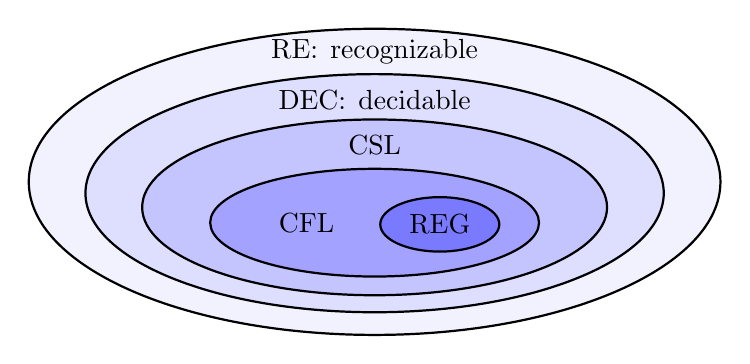
\begin{tikzpicture}[scale=0.72]
    \draw[thick,fill=blue!5] (0,0) ellipse (6.1 and 2.7);
    \node at (0,2.3) {$\RE$: recognizable};
    \draw[thick,fill=blue!13] (0,-0.2) ellipse (5.1 and 2.1);
    \node at (0,1.45) {$\mathrm{DEC}$: decidable};
    \draw[thick,fill=blue!23] (0,-0.45) ellipse (4.1 and 1.55);
    \node at (0,0.65) {$\mathrm{CSL}$};
    \draw[thick,fill=blue!36] (0,-0.72) ellipse (2.9 and 0.95);
    \node at (-1.2,-0.72) {$\mathrm{CFL}$};
    \draw[thick,fill=blue!52] (1.15,-0.75) ellipse (1.05 and 0.48);
    \node at (1.15,-0.75) {$\mathrm{REG}$};
  \end{tikzpicture}
  \end{center}
  $\mathrm{CSL}\subseteq\mathrm{DEC}$ follows from finite configuration
  search. Strictness requires a space-hierarchy/diagonalization argument;
  it does not follow merely because TMs have more available tape.
\end{frame}

% ==========================================
% Part 6: Computational Complexity
% ==========================================
\section{Computational Complexity: \texorpdfstring{$P$ and $NP$}{P and NP}}

\begin{frame}{From Computability to Complexity}
  \small
  Complexity theory studies the resources used by \emph{deciders}, usually as a function of input
  length $n$ and in the worst case.
  \begin{block}{Time complexity}
    $\mathrm{TIME}(t(n))$ is the class of languages decidable by a deterministic TM in
    $O(t(n))$ steps.
  \end{block}
  \begin{block}{The class $P$}
    \[
      P=\bigcup_{k\ge1}\mathrm{TIME}(n^k).
    \]
    Thus $P$ contains languages decidable in polynomial time on a deterministic TM.
  \end{block}
  DFA membership and directed graph reachability are examples in $P$.
  The appendix gives further examples and closure proofs.
  \par\smallskip
  $P$ is a robust mathematical model of efficient computation, but ``polynomial'' is not identical
  to ``fast in practice'': constants, exponents, input sizes, and machine models still matter.
\end{frame}


\begin{frame}{The Class $NP$: Verifiers and Certificates}
  \small
  A language $L$ lies in $NP$ iff there are a polynomial-time verifier $V$ and polynomial $p$ such that
  \[
    x\in L
    \iff
    \exists c,\ |c|\le p(|x|)\text{ and }V(x,c)=1.
  \]
  Equivalently, $NP$ is the class decidable in polynomial time by an NTM.
  \begin{block}{Example: $\mathrm{CLIQUE}$}
    Instance: a simple undirected graph $G$ and nonnegative integer $k$.
    Certificate: $k$ \emph{distinct} vertex identifiers from $G$.
    Reject $k>|V(G)|$; verify every pair is joined by an edge.
    The certificate has polynomial length even when $k$ is encoded in binary.
  \end{block}
  \begin{alertblock}{Mnemonic}
    $NP$ means \textbf{nondeterministic polynomial time}, not ``non-polynomial.''
    We know $P\subseteq NP$.
  \end{alertblock}
  $V$ must halt in time polynomial in $|x|+|c|$ on every pair. Checking
  one proposed certificate is different from finding a successful one.
\end{frame}

\begin{frame}{Polynomial-Time Reductions and NP-Completeness}
  \small
  $A\le_p B$ means there is a polynomial-time computable $f$ satisfying
  $x\in A\iff f(x)\in B$.
  \begin{itemize}
    \item $B$ is \textbf{NP-hard} if every $A\in NP$ reduces to $B$.
    \item $B$ is \textbf{NP-complete} if $B\in NP$ and $B$ is NP-hard.
  \end{itemize}
  \begin{block}{Standard proof strategy}
    To prove a new problem $B$ NP-complete:
    \begin{enumerate}
      \item show $B\in NP$ by giving a verifier;
      \item choose a known NP-complete problem $A$; and
      \item construct and prove a polynomial reduction $A\le_p B$.
    \end{enumerate}
  \end{block}
  Again, reducing $B$ to a known hard problem does not establish that $B$ is hard.
  \begin{block}{Anchor theorem: Cook--Levin and its 3SAT corollary}
    SAT (satisfiable Boolean formulas) and 3SAT (satisfiable conjunctions
    of three-literal clauses) are NP-complete. Thus a polynomial-time
    algorithm for either would imply $P=NP$. Proof sketches and a worked
    reduction to CLIQUE are in the appendix.
  \end{block}
\end{frame}



\begin{frame}{The $P$ versus $NP$ Question}
  \small
  \begin{columns}[T]
    \column{0.48\textwidth}
    \centering
    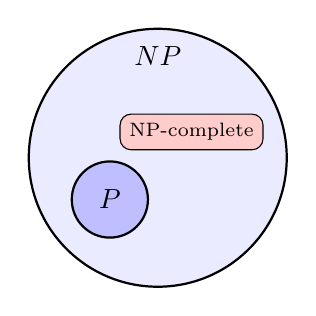
\begin{tikzpicture}[scale=0.78]
      \draw[thick,fill=blue!8] (0,0) circle (2.1);
      \node at (0,1.65) {$NP$};
      \draw[thick,fill=blue!25] (-0.78,-0.68) circle (0.62);
      \node at (-0.78,-0.68) {$P$};
      \node[draw,fill=red!20,rounded corners,font=\scriptsize] at (0.55,0.42) {NP-complete};
    \end{tikzpicture}

    If $P\ne NP$, no NP-complete language is in $P$.

    \column{0.48\textwidth}
    \centering
    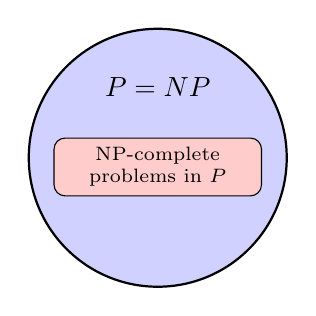
\begin{tikzpicture}[scale=0.78]
      \draw[thick,fill=blue!18] (0,0) circle (2.1);
      \node at (0,1.15) {$P=NP$};
      \node[draw,fill=red!20,rounded corners,text width=2.4cm,align=center,
        font=\scriptsize]
        at (0,-0.15) {NP-complete problems in $P$};
    \end{tikzpicture}

    If $P=NP$, all NP problems have polynomial-time algorithms.
  \end{columns}
  \vspace{0.2cm}
  The question remains open~\cite{clay-pnp}. Every $NP$ language is decidable:
  enumerate the finitely many certificates of permitted length and run the
  verifier on each. This may require far more than polynomial time.
  The issue is efficiency, not computability.
\end{frame}

\begin{frame}{Common Conceptual Traps}
  \small
  \begin{center}
  \begin{tabular}{L{4.4cm}L{6.0cm}}
    \toprule
    Misconception & Correction \\
    \midrule
    ``Undecidable means the program is slow.'' & No algorithm halts with the correct answer on every input. \\
    ``Recognizable means decidable.'' & A recognizer may loop on nonmembers. \\
    ``Nondeterministic means random.'' & Acceptance is existential over computation branches. \\
    ``NP means not polynomial.'' & $NP$ means nondeterministic polynomial time; $P\subseteq NP$. \\
    ``NP-complete means undecidable.'' & NP-complete problems are decidable, often by exponential-time search. \\
    ``A more convenient TM is more powerful.'' & Multitape and nondeterministic TMs have the same computability power. \\
    \bottomrule
  \end{tabular}
  \end{center}
\end{frame}

% ==========================================
% Review
% ==========================================
\section{Review and Exercises}

\begin{frame}{Checkpoint Exercises I: TMs and Decidability}
  \begin{enumerate}
    \item Does adding a stay-put move $S$ increase a TM's language-recognition power? Explain a simulation.
    \item Give a high-level decider for $\{w\#w\mid w\in\{0,1\}^*\}$.
    \item Contrast $A_{\mathrm{DFA}}$ with $\ATM$. Why does direct simulation decide one but only recognize the other?
    \item Suppose both $L$ and $\overline L$ have recognizers. Construct a decider for $L$.
    \item Is every undecidable language unrecognizable? Give a counterexample.
  \end{enumerate}
\end{frame}

\begin{frame}{Checkpoint Exercises II: Reductions and Complexity}
  \begin{enumerate}
    \item To prove a new problem $B$ undecidable using $\ATM$, which direction should the reduction go?
    \item Is ``$L(M)$ contains at least five strings'' covered by Rice's theorem? Is ``$M$ has at least five states''?
    \item Prove that $P$ is closed under complement.
    \item Is $NP$ known to be closed under complement?
    \item What two obligations must be met to prove that a problem is NP-complete?
    \item Why would a polynomial-time algorithm for $3\mathrm{SAT}$ imply $P=NP$?
  \end{enumerate}
\end{frame}

\begin{frame}{Checkpoint Exercises III: Bounded Space and Encodings}
  \small
  \begin{enumerate}
    \item On $aabbccc$, what is the tape after two rounds of the LBA's
      matching routine? Why must the final check reject?
    \item An LBA has $4$ states, $3$ interior cells, $2$ possible symbols
      per interior cell, and two fixed endmarkers. Give a configuration
      upper bound when the head may also scan either marker.
    \item One branch of an NLBA repeats a configuration. Must the input
      be rejected? Contrast this with a deterministic run.
    \item Why does deciding membership for each fixed LBA input not decide
      whether its language is empty?
    \item A proposed reduction simulates $M(w)$ to completion \emph{before}
      producing its output. What can go wrong?
  \end{enumerate}
  Write down the quantifiers: a statement about \emph{one} input is not
  automatically a statement about \emph{all} input lengths.
\end{frame}

\begin{frame}{Summary}
  \small
  \begin{itemize}
    \item CSGs correspond to nondeterministic LBAs; bounded-input configuration
      search makes every CSL decidable, but not necessarily easy to decide.
    \item TMs provide a robust formal model of algorithms and unrestricted computation.
    \item Deciders halt on all inputs; recognizers may loop on nonmembers.
    \item $\ATM$ is recognizable but undecidable; diagonalization and reductions expose this limit.
    \item Mapping reductions transfer decidability and recognizability results in a precise direction.
    \item Rice's theorem covers every nontrivial semantic property of a TM's recognized language.
    \item Complexity asks how many resources decidable problems require; $P$ versus $NP$ remains open.
  \end{itemize}
\end{frame}

\appendix
\section{Appendix: Challenges, Constructions, and Further Results}

\begin{frame}{Appendix Guide}
  \small
  The core sequence retains the CSG/LBA bridge, TM design, diagonalization,
  mapping reductions, Rice's theorem, and the definitions of $P$ and $NP$.
  Select appendix material according to course depth:
  \begin{itemize}
    \item CSG examples, finite configuration graphs, and LBA emptiness;
    \item a complete transition table, multitape simulation, and termination;
    \item checkpoint answers and five solved construction/proof challenges;
    \item Rice's theorem, TM equivalence, and different kinds of reduction;
    \item closure of $P$, Cook--Levin, SAT-to-3SAT, and 3SAT-to-CLIQUE.
  \end{itemize}
  The six relocated enrichment frames are retained in full. Attempt each
  challenge before reading its solution; the source guide distinguishes
  edition-specific textbook problems from newly phrased course practice.
  Check the acceptance mode, encoding, quantifiers, and reduction direction.
\end{frame}

\subsection{Context-Sensitive Grammars and Bounded Space}

\begin{frame}{Separate Counts Are Not the Same as One Shared Count}
  \small
  Compare two four-block languages:
  \begin{block}{Context-free: two independent adjacent matches}
    $L_1=\{a^nb^nc^md^m:n,m\ge0\}$ has the CFG
    \[
      S\to AB,\qquad A\to aAb\mid\varepsilon,
      \qquad B\to cBd\mid\varepsilon.
    \]
    A PDA finishes matching $a$'s against $b$'s, then reuses its stack
    for the $c$'s and $d$'s.
  \end{block}
  \begin{block}{Context-sensitive but not context-free: one count shared four ways}
    $L_2=\{a^nb^nc^nd^n:n\ge0\}$ is checked by four-way marking on an LBA.
    If it were a CFL, the homomorphism deleting $d$ and retaining $a,b,c$
    would make $\{a^nb^nc^n:n\ge0\}$ a CFL, a contradiction.
  \end{block}
  Here we use CFL closure under homomorphism from Slide Set 5.
  For $L_2$, accept $\varepsilon$ separately before checking nonempty blocks.
\end{frame}

\begin{frame}{A Noncontracting Grammar for Three Equal Blocks}
  \small
  For $\{a^nb^nc^n:n\ge1\}$, use variables $S,B,C$ and rules
  \[
    \begin{aligned}
      S&\to aSBC\mid aBC, & CB&\to BC,\\
      aB&\to ab, & bB&\to bb,\\
      bC&\to bc, & cC&\to cc.
    \end{aligned}
  \]
  All rules are noncontracting; the swap $CB\to BC$ is not itself in
  context-preserving form. The language-equivalence theorem relates the
  two grammar definitions.
  \begin{block}{Deriving $aabbcc$}
    \[
      \begin{aligned}
        S&\Rightarrow aSBC\Rightarrow aaBCBC\Rightarrow aaBBCC\\
         &\Rightarrow aabBCC\Rightarrow aabbCC
          \Rightarrow aabbcC\Rightarrow aabbcc.
      \end{aligned}
    \]
  \end{block}
  Each $S$ expansion supplies one $a,B,C$. Swaps preserve these counts;
  terminalization preserves them too. A terminal derivation must have all
  $b$'s before all $c$'s: a $B$ stranded to the right of a terminal $c$
  cannot be converted. Conversely, sort $(BC)^n$ to $B^nC^n$ before
  terminalizing to obtain every $a^nb^nc^n$.
\end{frame}

\begin{frame}{How Many Configurations Can an LBA Have?}
  \small
  Fix an LBA $B$ and an input $w$ of length $n$. In our convention, there
  are $n$ writable cells and two fixed marker cells. Let $g$ be the number
  of symbols allowed in an interior cell. A configuration specifies:
  \[
    \underbrace{|Q|}_{\text{state}}\ \times\
    \underbrace{(n+2)}_{\text{head position}}\ \times\
    \underbrace{g^n}_{\text{interior tape contents}}
    \ =:\ C.
  \]
  This is an upper bound; many configurations may be unreachable.
  If markers and their head positions are excluded by another convention,
  the often-quoted bound is $|Q|ng^n$ instead.
  \begin{block}{Deterministic halting on one given input}
    Simulate the unique run, stopping if it halts. If $C+1$ configurations
    have been visited without halting, some repeats. Determinism forces
    the same future, so this run loops forever. Alternatively, store
    visited configurations and detect repetition directly.
  \end{block}
  For $|Q|=4,n=3,g=2$, the bound is $4\cdot5\cdot8=160$.
  It also handles $n=0$: the head can still scan either marker.
\end{frame}

\begin{frame}{For an NLBA, Search a Graph---Not One Branch}
  \small
  For fixed $(B,w)$, create a vertex for each reachable configuration and
  an edge for each legal step. Treat accepting and blocked configurations
  as terminal. The graph is finite even if some runs are infinite.
  \begin{center}
  \begin{tabular}{L{4.5cm}L{5.8cm}}
    \toprule
    Question about this input & Finite-graph test \\
    \midrule
    Is $w$ accepted? & Is an accepting configuration reachable? \\
    Does some branch halt? & Is any terminal configuration reachable? \\
    Do all branches halt? & Is the reachable nonterminal subgraph acyclic? \\
    \bottomrule
  \end{tabular}
  \end{center}
  A reachable cycle can support an infinite branch \emph{and} have an exit
  leading to acceptance. Thus one repeated configuration on one branch
  is not a rejection certificate for an NLBA.
  \begin{block}{Consequence}
    $A_{\mathrm{LBA}}=\{\langle B,w\rangle:B\text{ accepts }w\}$ is decidable.
    Hence every CSL is decidable. The external graph-search decider need
    not itself obey the LBA's linear space restriction.
  \end{block}
\end{frame}

\begin{frame}{The Catch: LBA Emptiness Is Undecidable}
  \small
  \[
    E_{\mathrm{LBA}}=\{\langle B\rangle:L(B)=\emptyset\}.
  \]
  Finite configuration search settles one $(B,w)$, not every possible
  input length. There is no fixed global finite graph covering all inputs.
  \begin{block}{Computation-history reduction \cite{sipser-history}}
    Given $\langle M,w\rangle$, construct an LBA $B$ whose input is a
    proposed finite accepting computation history of $M$ on $w$.
    Check the initial configuration, each consecutive transition, and
    the accepting final configuration; reject malformed histories.
    \par\smallskip
    These checks compare finite fields by sweeps and marks within the
    supplied history. Fixed extra tracks can be packed into the tape alphabet.
    Thus $B$ can even be deterministic and halt on every history it checks.
  \end{block}
  There is an accepted history iff $M$ accepts $w$, so
  \[
    \ATM\le_m\overline{E_{\mathrm{LBA}}}.
  \]
  A decider for emptiness, with its answer reversed, would decide $\ATM$.
  Malformed source encodings map to a fixed empty-language LBA.
  This does not contradict decidable membership for every individual CSL.
\end{frame}

\begin{frame}{Optional Complexity: LBA Acceptance and PSPACE}
  \small
  $\mathrm{PSPACE}$ consists of decision languages solvable by a deterministic
  TM in space polynomial in the encoded input length.
  \begin{block}{Uniform acceptance problem \cite{lba-complexity}}
    $A_{\mathrm{LBA}}$ is PSPACE-complete: the input contains \emph{both}
    the LBA description and its word, with the tape bound enforced by the
    model. This is not a claim about every individual fixed CSL.
  \end{block}
  \textbf{Why polynomial space suffices:} one configuration and a counter
  up to $C$ take polynomial space. Guess a path of length less than $C$;
  Savitch's theorem converts this nondeterministic polynomial-space test
  to a deterministic polynomial-space one.
  \par\smallskip
  \textbf{Why it is hard:} a polynomial-space decider can be simulated
  on an LBA input padded to supply its polynomially many tape cells.
  The padding and machine description are constructible in polynomial time.
  \par\smallskip
  Deterministic-LBA halting is PSPACE-complete as well: for hardness,
  modify this simulation to halt on acceptance and loop on rejection.
  A large configuration bound alone proves neither PSPACE-hardness nor
  an unconditional exponential-time lower bound.
\end{frame}

\subsection{Machine Models and Termination}

\begin{frame}{A Complete Small TM: Scan and Flip Bits}
  \small
  Let $Q=\{q_s,q_{\mathrm{accept}},q_{\mathrm{reject}}\}$,
  $\Sigma=\{0,1\}$, $\Gamma=\{0,1,\sqcup\}$, and start in $q_s$.
  These are \emph{all} transitions on nonhalting states:
  \[
    \begin{array}{c|ccc}
      \text{scanned symbol}&0&1&\sqcup\\\hline
      \delta(q_s,\cdot)&(q_s,1,R)&(q_s,0,R)&(q_{\mathrm{accept}},\sqcup,R)
    \end{array}
  \]
  On $01$, the configurations are
  \[
    q_s01\ \vdash\ 1q_s1\ \vdash\ 10q_s\sqcup
    \ \vdash\ 10\sqcup q_{\mathrm{accept}}\sqcup.
  \]
  \begin{block}{Two questions about the same machine}
    As a \emph{recognizer}, it accepts $\{0,1\}^*$, including $\varepsilon$.
    As a \emph{string transformer}, with the output taken before the first
    blank, it computes bitwise complementation: $01\mapsto10$.
  \end{block}
  For $0\le r\le|w|$, after $r$ steps exactly the first $r$ bits have been flipped.
  The first blank is reached after $|w|$ steps; one further step accepts.
  An unreachable reject state is allowed.
\end{frame}

\begin{frame}{Multitape Turing Machines}
  \small
  A $k$-tape TM has $k$ tapes and $k$ independently moving heads:
  \[
    \delta:(Q\setminus\{q_{\mathrm{accept}},q_{\mathrm{reject}}\})
    \times\Gamma^k\to Q\times\Gamma^k\times\{L,R,S\}^k.
  \]
  \begin{block}{Theorem}
    Every multitape TM has an equivalent single-tape TM.
  \end{block}
  \textbf{Proof sketch.}
  Encode the $k$ virtual tapes as delimited regions on one tape and decorate each region's scanned
  symbol to record its virtual head. One simulated step uses sweeps to read all head symbols,
  update them, and move the head markers.

  If the multitape machine runs in time $t(n)\ge n$, with $k$ fixed,
  the standard simulation takes
  $O(t(n)^2)$ time after accounting for the single tape's repeated sweeps.
  \begin{alertblock}{Interpretation}
    Same computability, potentially different running time. Model robustness does not mean equal speed.
  \end{alertblock}
\end{frame}

\begin{frame}{Why a Halting NTM Has a Finite Computation Tree}
  \small
  Fix one input and unfold its computations into a rooted tree: a node is
  a computation prefix, and its children are the finitely many next moves.
  \begin{block}{K\"onig's lemma: the relevant form}
    Every infinite, finitely branching rooted tree has an infinite branch.
  \end{block}
  \textbf{Proof idea:} if the root has infinitely many descendants, one of
  its finitely many children must have infinitely many descendants. Choose
  such a child repeatedly; the choices build an infinite branch.
  \par\smallskip
  Therefore, if \emph{every} computation branch halts, the tree must be
  finite. Breadth-first simulation eventually exhausts it, accepting if
  any branch accepts and otherwise rejecting.
  \begin{alertblock}{Where the hypotheses matter}
    Infinitely many finite branches need not have bounded depth in an
    \emph{infinitely branching} tree. TMs avoid that issue because their
    transition descriptions have finite branching. For a recognizer with
    an infinite branch, breadth-first search need not terminate on a nonmember.
  \end{alertblock}
  A finite tree for each input establishes termination, not a polynomial
  running-time bound.
\end{frame}

\subsection{Worked Checkpoint Answers}

\begin{frame}{Solutions I: TMs and Decidability}
  \small
  \begin{enumerate}
    \item Simulate $(q,a)\mapsto(p,b,S)$ by writing $b$ and moving right
      to a helper state; preserve the encountered symbol, move left, and
      enter $p$. Moving right first also works at the left boundary.
    \item For $w\#w$, check that exactly one $\#$ occurs. Mark the next
      unmarked bit in the left half, remember it in finite control, and
      match the next unmarked bit on the right. Reject mismatches or
      unequal lengths. Accept when both halves are exhausted, including
      the input $\#$. Each round marks new cells, so the procedure halts.
    \item A DFA consumes exactly one symbol per step, so its run finishes
      after $|w|$ steps. A simulated TM may continue forever.
    \item Alternate steps of the two recognizers. Accept if the $L$
      recognizer accepts; reject if the $\overline L$ recognizer accepts.
      Exactly one event must eventually occur.
    \item No. $\ATM$ is recognizable but undecidable.
  \end{enumerate}
\end{frame}

\begin{frame}{Solutions II: Reductions and Complexity}
  \small
  \begin{enumerate}
    \item Use $\ATM\le_m B$: a hypothetical decider for $B$ would decide
      the known undecidable source.
    \item ``At least five strings'' is semantic and nontrivial:
      $\emptyset$ fails and $\Sigma^*$ satisfies it. ``At least five states''
      is syntactic and can be checked directly from the description.
    \item Swap the two halting outcomes of a polynomial-time decider;
      its running time is unchanged.
    \item It is not known whether $NP$ is closed under complement;
      this is equivalent to $NP=\mathrm{coNP}$. Here
      $\mathrm{coNP}=\{L:\overline L\in NP\}$. Do not confuse this with
      $P$'s known complement closure.
    \item Prove both $B\in NP$ and NP-hardness. For the latter, reduce
      a known NP-complete language \emph{to} $B$ in polynomial time.
    \item Every $A\in NP$ reduces to 3SAT in polynomial time. Composing
      that reduction with a polynomial-time 3SAT decider puts $A$ in $P$.
      Together with $P\subseteq NP$, this gives $P=NP$.
  \end{enumerate}
\end{frame}

\begin{frame}{Solutions III: Bounded Space and Encodings}
  \small
  \begin{enumerate}
    \item The interior is $XXYYZZc$. The final scan finds an unmatched
      $c$ and rejects; seeing no unmarked $a$ alone is not enough.
    \item $4(3+2)2^3=160$ configurations at most, including head positions
      on the two endmarkers.
    \item Not necessarily: another branch may accept, or a later choice
      may exit the cycle. In a deterministic run, repeating a nonhalting
      configuration forces the same infinite future.
    \item Emptiness asks whether \emph{any} word of \emph{any} length
      is accepted. Testing words one by one can find a witness to
      nonemptiness but cannot generally certify its absence.
    \item If $M(w)$ loops, that translator never outputs anything, so it
      is not a total mapping reduction. Write a program containing the
      simulation instead; the translator itself must always terminate.
  \end{enumerate}
  In all three topics, distinguish the finite description of a process
  from the potentially infinite behavior of the process it describes.
\end{frame}

\subsection{Solved Challenges: Enumeration, Machines, and Search}

\begin{frame}{Challenge Sources and Study Route}
  \small
  These prompts are paraphrased, with worked arguments written for this
  course. Exercise numbers depend on the edition.
  \begin{center}
  \begin{tabular}{L{5.6cm}L{4.8cm}}
    \toprule
    Challenge & Source / status \\
    \midrule
    1. Ordered enumeration and decidability & Sipser, 3rd ed., Problem 3.18 \\
    2. An infinite decidable subset & Sipser, 3rd ed., Problem 3.19 \\
    3. An effective list of deciders is incomplete & Sipser, 3rd ed., Problem 4.30 \\
    4. A head that may move right or stay & Sipser, 2nd ed., Problem 3.13 \\
    5. Find a SAT witness using a decision procedure & Additional course practice;
      no numbered exercise claimed \\
    \bottomrule
  \end{tabular}
  \end{center}
  University sources verify the numbered prompts~\cite{challenge-enumerators,challenge-machines}.
  Linz's construction viewpoint supports Challenge 4; Sipser's enumeration
  and diagonalization viewpoint guides Challenges 1--3.
  \begin{block}{Questions to ask before checking the solution}
    What guarantees progress? Does the argument handle finite and empty
    languages? Does it prove that a decider exists, or give a uniform
    algorithm to obtain one from the supplied description?
  \end{block}
\end{frame}

\begin{frame}{Challenge 1: Ordered Enumeration and Decidability}
  \small
  \textbf{Sipser 3rd ed., Problem 3.18.} Show that $L$ is decidable iff
  some enumerator prints its words in increasing \emph{standard string order}.
  Here this means length first, then dictionary order (shortlex):
  \[
    \varepsilon,0,1,00,01,10,11,000,\ldots
  \]
  \begin{block}{Decider $\Rightarrow$ ordered enumerator}
    Visit all strings in shortlex order. Run the decider on each and print
    exactly those it accepts. Every test halts, so every word of $L$
    is eventually printed, in order.
  \end{block}
  \begin{block}{Ordered enumerator $\Rightarrow$ existence of a decider}
    If $L$ is infinite, on input $x$ simulate the enumerator until it prints
    $x$ (accept) or a word after $x$ (reject). There are only finitely many
    words at or before $x$, so one event must occur.
    \par\smallskip
    If $L$ is finite, it is decidable by a finite membership table, including
    the empty-table case. This is a separate case, not the same simulation.
  \end{block}
  A finite-language enumerator may run silently forever after its last
  output. The theorem does not supply an end-of-enumeration test.
\end{frame}

\begin{frame}{A Subtle Point: Existence Is Not Uniform Construction}
  \small
  Challenge 1 does \emph{not} give an algorithm that converts every
  ordered enumerator into a decider for its language.
  \begin{block}{Why such a general converter cannot exist}
    From $\langle M,w\rangle$, effectively build an enumerator $E$ that
    simulates $M(w)$ and prints $\varepsilon$ only if that simulation accepts.
    It prints nothing otherwise. Its language is either
    $\{\varepsilon\}$ or $\emptyset$, and in either case its outputs are ordered.
    \par\smallskip
    A supposed converter would produce a decider $D_E$. Running
    $D_E(\varepsilon)$ would then decide whether $M$ accepts $w$,
    contradicting the undecidability of $\ATM$.
  \end{block}
  Both possible languages individually have easy deciders; the impossible
  task is choosing the correct one \emph{effectively from this description}.
  \par\smallskip
  Under the additional promise that the enumerated language is infinite,
  the simulation from Challenge 1 \emph{is} a uniform construction.
  This distinction also explains why infinitely many decidable fixed-input
  cases need not yield a decision procedure for a uniform problem.
\end{frame}

\begin{frame}{Challenge 2: An Infinite Decidable Subset}
  \small
  \textbf{Sipser 3rd ed., Problem 3.19.} Prove that every infinite
  recognizable language $L$ contains an infinite decidable subset $B$.
  \begin{block}{Construction: retain only new length records}
    Run an enumerator for $L$. Retain its first output; thereafter retain
    an output only when its length is strictly greater than the length of
    the last retained word. Let $B$ be the set of retained words.
  \end{block}
  \textbf{Subset and infinitude.} Every retained word belongs to $L$.
  Over a finite alphabet, only finitely many words have bounded length.
  Since $L$ is infinite, longer outputs keep appearing; hence $B$ is infinite.
  \par\smallskip
  \textbf{Decider for $B$.} On input $x$, simulate the retention process.
  Accept if it retains $x$; reject once it retains a word longer than $x$.
  Retained lengths are strictly increasing and unbounded, so this halts.
  \begin{alertblock}{Do not test against every output of the original enumerator}
    Only retained words belong to $B$. A discarded output equal to $x$
    does not justify acceptance. Also, this result does not make $L$
    decidable: an undecidable language may contain an easy infinite subset.
  \end{alertblock}
\end{frame}

\begin{frame}{Challenge 3: No Effective List Covers All Decidable Languages}
  \small
  \textbf{Sipser 3rd ed., Problem 4.30.} Let $A$ be a recognizable set
  of TM descriptions over a fixed input alphabet, each describing a decider.
  Show that some decidable
  language is not decided by any machine whose description belongs to $A$.
  \begin{block}{Diagonal construction when $A$ is infinite}
    Enumerate its distinct descriptions as $\langle M_0\rangle,
    \langle M_1\rangle,\ldots$, suppressing repeats. List all input words
    $w_0,w_1,\ldots$ in shortlex order. Define a machine $D$:
    \begin{enumerate}
      \item On $w_i$, enumerate until $M_i$ appears.
      \item Run $M_i$ on $w_i$ and reverse its accept/reject answer.
    \end{enumerate}
  \end{block}
  The enumeration reaches its $i$th distinct description because $A$ is
  infinite; $M_i$ halts because it is a decider. Thus $D$ is a decider,
  but $L(D)\ne L(M_i)$ for every $i$, witnessed by $w_i$.
  \par\smallskip
  If $A$ is finite, its machines decide only finitely many languages;
  choose a singleton language not among them.
  \par\smallskip
  All TM descriptions can be listed, but no effective list containing
  \emph{only deciders} can represent every decidable language.
\end{frame}

\begin{frame}{Challenge 4: Remove Left Moves, Lose Language Power}
  \small
  \textbf{Sipser 2nd ed., Problem 3.13.} A deterministic TM may write,
  move right, or stay, but never move left. Show it recognizes only regular
  languages, even though its tape is unbounded.
  \begin{block}{Summarize processing of one cell}
    Starting with state $q$ and scanned symbol $a$, simulate stay moves
    until the machine accepts, rejects, moves right in state $p$, or
    repeats a state/symbol pair. Repetition implies a local infinite loop;
    there are at most $|Q||\Gamma|$ such pairs.
  \end{block}
  Make these summaries the transitions of a DFA. Early acceptance goes
  to an accepting sink; rejection or local looping goes to a rejecting sink.
  A right move goes to $p$: abandoned tape cells can never be read again.
  \par\smallskip
  After input ends, the TM may traverse fresh blank cells. Summarize each
  blank-cell visit similarly; only finitely many entry states exist.
  Mark a DFA state final iff this blank-only continuation eventually accepts.
  Thus the DFA has exactly the same language. Conversely, a right-moving
  TM can simulate any DFA and decide at the first blank.
  \par\smallskip
  Adding stay moves to $L/R$ changes no power; \emph{replacing} left by stay does.
\end{frame}

\begin{frame}{Challenge 5: Find a SAT Witness Using Yes/No Answers}
  \small
  \textbf{Additional practice:} given a polynomial-time SAT decider $D$,
  construct a polynomial-time algorithm that returns a satisfying assignment
  for a formula $\varphi$, or reports that none exists.
  \begin{enumerate}
    \item Ask $D(\varphi)$. If the answer is no, report unsatisfiable.
    \item Maintain a partial assignment with a satisfying extension.
      For each unassigned variable $x_i$, ask whether
      $\varphi$ together with the current assignments and $x_i=0$ is satisfiable.
    \item If yes, keep $x_i=0$; otherwise set $x_i=1$.
      Continue until every variable is assigned.
  \end{enumerate}
  \begin{block}{Why the invariant survives}
    Before each query, at least one extension exists. Such an extension
    sets $x_i$ either to 0 or to 1. If the 0 branch has no extension, the
    1 branch must have one. The final complete assignment therefore satisfies
    $\varphi$.
  \end{block}
  For $m$ variables, at most $m+1$ queries are made; appended assignment
  constraints keep every query polynomial in the original input size.
  This is an adaptive \emph{search-to-decision} reduction, not a single
  mapping reduction between two decision languages.
\end{frame}

\subsection{Undecidability and Complexity Proof Sketches}

\begin{frame}{A Reduction That Also Shows Unrecognizability}
  \small
  Let $\ETM=\{\langle N\rangle:L(N)=\emptyset\}$.
  Given a valid $\langle M,w\rangle$, output a machine $N$ that on input $x$
  simulates $M(w)$ and accepts $x$ only if that simulation accepts.
  \[
    L(N)=
    \begin{cases}
      \Sigma^*,&M\text{ accepts }w,\\
      \emptyset,&M\text{ does not accept }w.
    \end{cases}
  \]
  Map malformed source strings to a fixed machine with empty language.
  The map is total and satisfies
  \[
    \overline{\ATM}\le_m\ETM.
  \]
  Since $\overline{\ATM}$ is unrecognizable, $\ETM$ is unrecognizable too:
  otherwise compute the map and run an $E_{\mathrm{TM}}$ recognizer.
  \begin{block}{But nonemptiness is recognizable}
    Dovetail $N$ on all strings and accept when any simulation accepts.
    Also accept malformed descriptions, since these belong to
    $\overline{\ETM}$ under our fixed encoding convention.
    Hence $\ETM$ is co-recognizable but not recognizable.
  \end{block}
\end{frame}

\begin{frame}{Rice's Theorem: Why the General Pattern Works}
  \small
  Let $\mathcal P$ be a nontrivial property of recognizable languages.
  First suppose $\emptyset\notin\mathcal P$; choose a recognizable
  language $K\in\mathcal P$ with recognizer $T$.
  \begin{block}{Construct a gated recognizer}
    Given $\langle M,w\rangle$, output $N$ whose action on $x$ is:
    simulate $M(w)$; if it accepts, run $T(x)$ and copy its outcome.
    If the first simulation rejects, reject; if it loops, keep simulating.
    \[
      L(N)=K\ \text{if }M\text{ accepts }w;
      \qquad L(N)=\emptyset\ \text{otherwise}.
    \]
  \end{block}
  Thus deciding whether $L(N)\in\mathcal P$ would decide $\ATM$.
  Invalid source encodings map to an empty-language machine.
  \par\smallskip
  If $\emptyset\in\mathcal P$, apply the argument to the complementary
  \emph{property} among recognizable languages and reverse the decision.
  This is not taking the complement of $K$ or claiming it is recognizable.
  \par\smallskip
  The proof uses both hypotheses: nontriviality supplies $K$, and
  semantic dependence makes the two language outcomes decisive.
\end{frame}

\begin{frame}{TM Equivalence: Neither Side Is Recognizable}
  \small
  Define $\mathrm{EQ}_{\mathrm{TM}}=\{\langle M_1,M_2\rangle:
  L(M_1)=L(M_2)\}$. Fix machines $E,U$ for $\emptyset,\Sigma^*$.
  From $\langle M,w\rangle$, construct $N$ that accepts its input exactly
  when the simulation of $M(w)$ accepts. Thus
  \begin{center}
  \begin{tabular}{lccc}
    \toprule
    Behavior of $M(w)$ & $L(N)$ & $L(N)=L(E)$? & $L(N)=L(U)$? \\
    \midrule
    accepts & $\Sigma^*$ & no & yes \\
    rejects or loops & $\emptyset$ & yes & no \\
    \bottomrule
  \end{tabular}
  \end{center}
  The two computable maps $\langle M,w\rangle\mapsto\langle N,E\rangle$
  and $\langle M,w\rangle\mapsto\langle N,U\rangle$ respectively establish
  \[
    \overline{\ATM}\le_m\mathrm{EQ}_{\mathrm{TM}},
    \qquad
    \overline{\ATM}\le_m\overline{\mathrm{EQ}_{\mathrm{TM}}}.
  \]
  For malformed source strings, use $N=E$; both equivalences still hold.
  Since $\overline{\ATM}$ is unrecognizable, neither target is recognizable.
  \begin{block}{Stronger than undecidability}
    There is no recognizer for all equivalent pairs, nor for all inequivalent
    pairs. Rice's theorem alone would not establish these two stronger claims.
    See Sipser's discussion of mapping reductions~\cite{sipser,sipser-notes}.
  \end{block}
\end{frame}

\begin{frame}{Mapping Reductions Are Not Oracle Reductions}
  \small
  Write $A\le_T B$ if an algorithm decides $A$ using a hypothetical
  \emph{oracle} that correctly answers membership queries for $B$.
  Queries may be adaptive; the oracle need not be computable.
  \begin{block}{An oracle can answer a question whose answer we then reverse}
    Always $A\le_T\overline A$: ask whether $x\in\overline A$ and flip
    the answer. A mapping reduction instead requires one total computable
    $f$ with $x\in A\iff f(x)\in B$; it cannot reverse that equivalence.
  \end{block}
  In fact, $\ATM\not\le_m\overline{\ATM}$. If such an $f$ existed, then
  \[
    x\notin\ATM\iff f(x)\in\ATM.
  \]
  Computing $f(x)$ and running an $\ATM$ recognizer would recognize
  $\overline{\ATM}$, a contradiction.
  \par\smallskip
  Hence $A\le_m B$ implies $A\le_T B$, but the converse fails.
  The SAT-witness challenge likewise uses several adaptive decision
  queries; it is not a single mapping reduction.
  \begin{alertblock}{State the reduction you are proving}
    Oracle access, a total computable translation, and a polynomial-time
    translation are different requirements. See~\cite{sipser}, Chapter~6.
  \end{alertblock}
\end{frame}

\subsection{Optional Complexity Constructions}

\begin{frame}{Examples and Closure Properties of $P$}
  \small
  $P$ is a class of \emph{decision languages}. Examples include:
  \begin{itemize}
    \item DFA membership and graph reachability;
    \item whether a graph with nonnegative binary-encoded integer weights
      has an $s$--$t$ path of weight at most $K$;
    \item whether an undirected weighted graph has a spanning tree of
      total weight at most $K$.
  \end{itemize}
  \begin{block}{Useful closure facts}
    $P$ is closed under union, intersection, concatenation, and complement.
  \end{block}
  Complement closure: run the decider and exchange accept with reject.
  For concatenation, try all $n+1$ splits $w=uv$ and run the two deciders;
  polynomially many polynomial-time tests remain polynomial.
  \par\smallskip
  Finding a shortest path or a minimum spanning tree is an associated
  function/optimization problem, also solvable in polynomial time.
  Complexity claims require an explicit encoding because $n$ is the length of that encoding.
\end{frame}

\begin{frame}{Cook--Levin Theorem: Why SAT Is NP-Complete}
  \begin{block}{Theorem}
    $\mathrm{SAT}$, the set of satisfiable Boolean formulas, is NP-complete.
  \end{block}
  \textbf{Membership in $NP$.} A truth assignment is a polynomial-size certificate and can be checked
  by evaluating the formula.

  \textbf{NP-hardness proof idea.} For any polynomial-time NTM computation, construct a Boolean
  formula describing a computation tableau. Variables encode the state, tape symbol, and head
  location at each time and tape position; local clauses enforce a legal start, transition sequence,
  and accepting state.
  \begin{alertblock}{Consequence}
    A polynomial-time algorithm for SAT---or for any NP-complete problem---would imply $P=NP$.
  \end{alertblock}
  The restriction 3SAT is also NP-complete. Fresh variables for subformulas
  convert SAT to clauses of at most three literals without exponential
  expansion; the next slide outlines this construction.
\end{frame}

\begin{frame}{SAT to 3SAT: Avoiding Exponential Expansion}
  \small
  Regard a formula as a tree of two-input AND/OR and one-input NOT gates.
  Introduce a fresh variable $z$ for each subformula's value.
  Enforce its relation to its children with constant-size clauses, e.g.
  \[
    z\leftrightarrow(x\land y)
    \quad\Longleftrightarrow\quad
    (\neg z\lor x)\land(\neg z\lor y)\land(z\lor\neg x\lor\neg y).
  \]
  For $z\leftrightarrow\neg x$, use $(z\lor x)\land(\neg z\lor\neg x)$;
  OR gates have analogous clauses. Add the unit clause asserting the root.
  \begin{block}{Why satisfiability is preserved}
    A satisfying assignment to the original variables extends by giving
    each new variable its subformula value. Conversely, the gate clauses
    force those values, and the root clause forces the original formula true.
  \end{block}
  Each clause has at most three literals. Repeating a literal pads short
  clauses to exactly three occurrences without changing their meaning.
  The number of variables and clauses is linear in the formula's tree size;
  writing their identifiers still takes only polynomial time~\cite{cnf-conversion}.
  \par\smallskip
  The new formula is \emph{equisatisfiable}, not logically equivalent over
  the enlarged variable set. This construction establishes SAT $\le_p$ 3SAT.
\end{frame}

\begin{frame}{A Concrete Polynomial Reduction: 3SAT to CLIQUE}
  \small
  Let $\varphi=C_1\land\cdots\land C_m$ have three literal occurrences
  per clause. Construct a graph with one vertex for each occurrence.
  \begin{enumerate}
    \item Put no edges between occurrences belonging to the same clause.
    \item Between different clauses, join two vertices exactly when their
      literals are not contradictory ($x$ and $\neg x$).
    \item Output $(G,k)$ with $k=m$.
  \end{enumerate}
  \begin{block}{The two directions}
    A satisfying assignment supplies one true literal per clause. These
    $m$ vertices are pairwise compatible, hence form a clique.
    \par\smallskip
    An $m$-clique uses one vertex from each clause. Its literals contain
    no contradictory pair, so assign them true and extend arbitrarily to
    other variables. Every clause then has a true literal.
  \end{block}
  There are $3m$ vertices and $O(m^2)$ candidate edges; comparing literal
  names also takes polynomial time in the formula encoding length.
  Since 3SAT is NP-complete and CLIQUE is in $NP$, CLIQUE is NP-complete.
  Malformed formulas map to a fixed no-instance: an empty graph with $k=1$.
\end{frame}

\subsection{References}

\begin{frame}{References: Numbered Challenge Sources}
  \footnotesize
  \setbeamertemplate{bibliography item}[text]
  \begin{thebibliography}{9}
    \bibitem[S06]{sipser-second}
      Michael Sipser, \emph{Introduction to the Theory of Computation},
      2nd ed., Thomson Course Technology, 2006.
      Problem~3.13: TMs with right and stay-put moves only.
    \bibitem[I22]{challenge-enumerators}
      University of Illinois Urbana--Champaign, CS~475, Spring 2022,
      \href{https://courses.grainger.illinois.edu/cs475/sp2022/ALL-lectures/Lectures/Day10.pdf}
      {\emph{Enumerators}}.
      Identifies Sipser Problems~3.18, 3.19, and 4.30 and clarifies
      the standard (shortlex) order of strings.
    \bibitem[T07]{challenge-machines}
      Luca Trevisan, UC Berkeley CS~172, February 12, 2007,
      \href{https://cs.stanford.edu/people/trevisan/cs172-07/hw4.pdf}
      {\emph{Problem Set 4}}.
      Identifies the second-edition right/stay-put machine problem.
  \end{thebibliography}
  Statements have been paraphrased and solutions developed for these slides.
  Use the edition-specific numbers in the challenge guide: exercise numbers
  can change between editions. The SAT-witness task and the uniform-conversion
  discussion are supplementary course material, not claimed numbered exercises.
\end{frame}

\begin{frame}{References: CSGs, LBAs, and Bounded Space}
  \footnotesize
  \setbeamertemplate{bibliography item}[text]
  \begin{thebibliography}{9}
    \bibitem[G]{gallier-csg}
      Jean Gallier, University of Pennsylvania,
      \href{https://www.cis.upenn.edu/~jean/gbooks/cis51104sl13pdf.pdf}
      {\emph{Phrase-Structure Grammars and Context-Sensitive Grammars}},
      Chapter 8. Context-preserving/noncontracting grammars and LBA equivalence.
    \bibitem[V]{lba-notes}
      VSB--Technical University of Ostrava, Introduction to Theoretical Informatics,
      \href{https://www.cs.vsb.cz/sawa/uti/slides/uti-06-en.pdf}
      {\emph{Turing Machines}}. LBA restrictions and the determinism question.
    \bibitem[S20]{sipser-history}
      Michael Sipser, MIT 18.404J, Fall 2020,
      \href{https://ocw.mit.edu/courses/18-404j-theory-of-computation-fall-2020/a48f01c5374e72ee4f68a70bc0e38583_MIT18_404f20_lec10.pdf}
      {Lecture 10: Computation History Method}.
      LBA acceptance versus emptiness and history checking.
    \bibitem[B21]{lba-complexity}
      UC Berkeley CS 172, Spring 2021,
      \href{https://people.eecs.berkeley.edu/~sinclair/cs172/sol9.pdf}
      {Problem Set 9 Solutions}.
      PSPACE-completeness of bounded-tape acceptance.
  \end{thebibliography}
\end{frame}

\begin{frame}{References: Computability and Complexity}
  \small
  \setbeamertemplate{bibliography item}[text]
  \begin{thebibliography}{9}
    \bibitem[MIT]{sipser-notes}
      Michael Sipser, MIT 18.404J, Fall 2020,
      \href{https://ocw.mit.edu/courses/18-404j-theory-of-computation-fall-2020/pages/lecture-notes/}
      {Lecture Notes}. Turing machines, undecidability, reductions,
      and complexity; Lecture 15 includes 3SAT $\le_p$ CLIQUE.
    \bibitem[E]{cnf-conversion}
      Jason Eisner, Johns Hopkins University,
      \href{https://www.cs.jhu.edu/~jason/tutorials/convert-to-CNF}
      {\emph{How to Convert a Formula to CNF}}.
      Fresh-variable encodings and equisatisfiability.
    \bibitem[CMI]{clay-pnp}
      Clay Mathematics Institute,
      \href{https://www.claymath.org/millennium/p-vs-np/}
      {\emph{P vs NP}}. Problem statement and open status;
      consulted September 2026.
  \end{thebibliography}
  The configuration-graph and reduction proofs here spell out the model
  and encoding conventions used in this slide set.
\end{frame}

\begin{frame}{References and Suggested Reading}
  \small
  \begin{thebibliography}{9}
    \bibitem{linz}
      Peter Linz and Susan H. Rodger,
      \newblock \emph{An Introduction to Formal Languages and Automata}, 7th ed.,
      \newblock Jones \& Bartlett Learning, 2023.

    \bibitem{sipser}
      Michael Sipser,
      \newblock \emph{Introduction to the Theory of Computation}, 3rd ed.,
      \newblock Cengage Learning, 2013.
  \end{thebibliography}
  \vspace{0.3cm}
  Recommended emphasis: Linz for machine construction and formal-language progression; Sipser for
  recognizability, diagonalization, reductions, and the verifier view of $NP$.
\end{frame}

\end{document}
